\chapter{Methodology}

\section{Acoustic Stored Product Insect Detection System (A-SPIDS)}

The Acoustic Stored Product Insect Detection System (A-SPIDS) was designed as a low-cost, portable, fast, and non-destructive alternative method to inspect stored products for insect infestations. The system is made up of a main body, an acoustically treated lid, and a base that provides vibration isolation and wireless charging to the integrated battery. The total system weighs \SI{9}{\kilo\gram} and has a length, height, and width of \SI{30}{\centi\meter}, \SI{24}{\centi\meter}, and \SI{19}{\centi\meter}, respectively. The body of the system is 3D-printed ABS plastic lined with \SI{1.875}{\centi\meter} thick acoustic foam and molded silicone. Figure \ref{fig:aspids_cad} shows an annotated rendered CAD model of A-SPIDS:

\begin{figure}[!htbp]
    \centering
    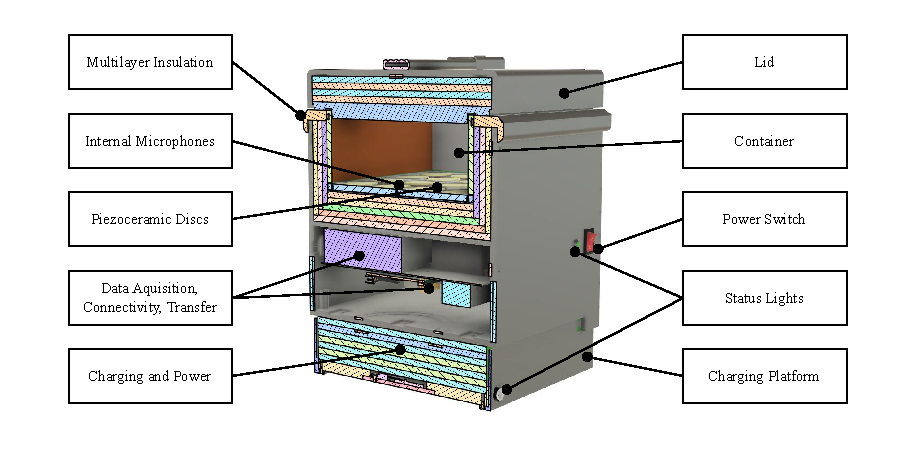
\includegraphics[width=\textwidth]{figures/methods/annotated_cad.pdf}
    \caption{Annotated rendered CAD model of A-SPIDS \label{fig:aspids_cad}}
\end{figure}

The main body features an integrated receptacle \SI{26}{\centi\meter} long, \SI{15}{\centi\meter} wide, and \SI{3.5}{\centi\meter} tall, capable of holding \SIrange{1}{1.5}{\litre} of product. The bottom of this receptacle is lined with 32 piezoelectric discs arranged in four groups of eight. This container size not only satisfies inspection sampling requirements but also stays within range for optimal insect detection based on the success of previous piezoelectric based sensors to detect the rice weevil, \textit{S. oryzae}, and the adult red flour beetle, \textit{T. castaneum}, in grain up to \SIrange{10}{15}{\centi\meter} and \SI{18.5}{\centi\meter} away, respectively, from the sensor \cite{vickSoundDetectionStoredProduct1988,hagstrumImprovingStoredProduct2019}. The maximum distance from the piezoelectric discs to any portion of the sample is set within the range even if the insects are active only on the surface of the substrate \cite{hagstrumEcologyIPMInsects2010}. 

\newpage
The discs are \SI{27}{\milli\meter} in diameter, \SI{0.33}{\milli\meter} thick, and made of piezoelectric ceramic lead zirconate titanate and brass \cite{PiezoelectricDiscDiameter2024}. The four groups correspond to channels zero through three in the recordings, complementary to their respective location in the system from left to right. The piezoelectric discs capture the mechanical sounds and vibrations generated by the insects moving, masticating, and mating within the product. Traditional acoustic microphones are placed throughout the body of the system to capture external noise and vibration. The microphones are POM-2735P-R with a diameter of \SI{6}{\milli\meter}, a height of \SI{4.7}{\milli\meter}, and a sensitivity of \SI{-35(2)}{\deci\bel} \cite{puiaudioPOM2735PRMicrophone2024}. Microphone channels four and five are colocated with the piezoelectric channels zero and one, respectively, while channel six is placed within the system body, and channel seven is mounted on the exterior of the system. Figure \ref{fig:aspids_sensor_diagram} shows the layout of the sensors.

\begin{figure}[!htbp]
	\centering
	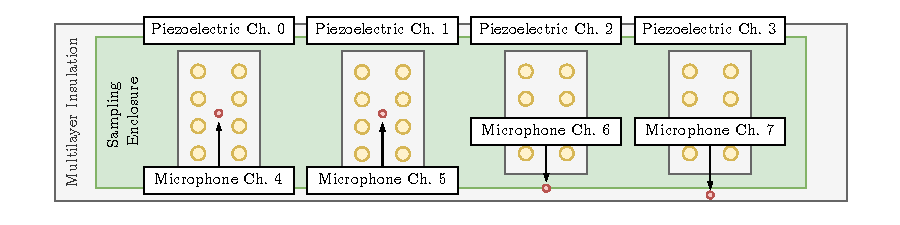
\includegraphics[width=\textwidth]{figures/methods/sensor_module_layout.pdf}
	\caption{Diagram of A-SPIDS sensor layout \label{fig:aspids_sensor_diagram}}
\end{figure}

The main body also contains the supportive hardware for data acquisition, communication, and power. The piezoelectric discs and microphones output to a proprietary amplifier and then converted to an I2S stream using a Texas Instruments PCM1808 analog-to-digital converter (ADC) \cite{PCM1808TexasInstruments}. The data is collected by a Raspberry Pi 3 A+ \cite{industriesRaspberryPiModel} and the I2S stream is digitized using a miniDSP MCHStreamer digital USB sound card \cite{MCHStreamerUSBAudio} with a \SI{24}{\kilo\hertz} sampling rate. The Raspberry Pi transmits data wirelessly to an aquisition computer through a Mikrotik mAP model RBmAP2nD \cite{MAPMikroTik}. The electronics are arranged on an electro-magnetic interference (EMI) shielding plate. Figure \ref{fig:aspids_elecronics_diagram} diagrams the electronics in A-SPIDS.

\begin{figure}[!htbp]
	\centering
	
\includegraphics[width=\textwidth]{figures/methods/electronics_layout.pdf}
	\caption{Diagram of A-SPIDS electronics \label{fig:aspids_elecronics_diagram}}
\end{figure}

An integrated battery can maintain the system for several hours and recharges using a receiver coil when positioned on the platform base which is powered by a \SI{24}{\volt} power supply. 

% The sensor can be lifted off and operated without the charging platform.

% During operation, the inspector places the sample material into the system enclosure and secures the lid. Unless the commodity is already packaged and portioned to \SIrange{1}{1.5}{\liter}, the product can be dispensed into a plastic bag. The inspector then initiates the data collection process until the system responds with the detection results. 

% Figure \ref{fig:aspids_photos} shows photographs of A-SPIDS in the closed and open configurations.

% \begin{figure}[!htbp]
% 	\centering
% 	\begin{subfigure}{0.45\textwidth}
% 		\centering
% 		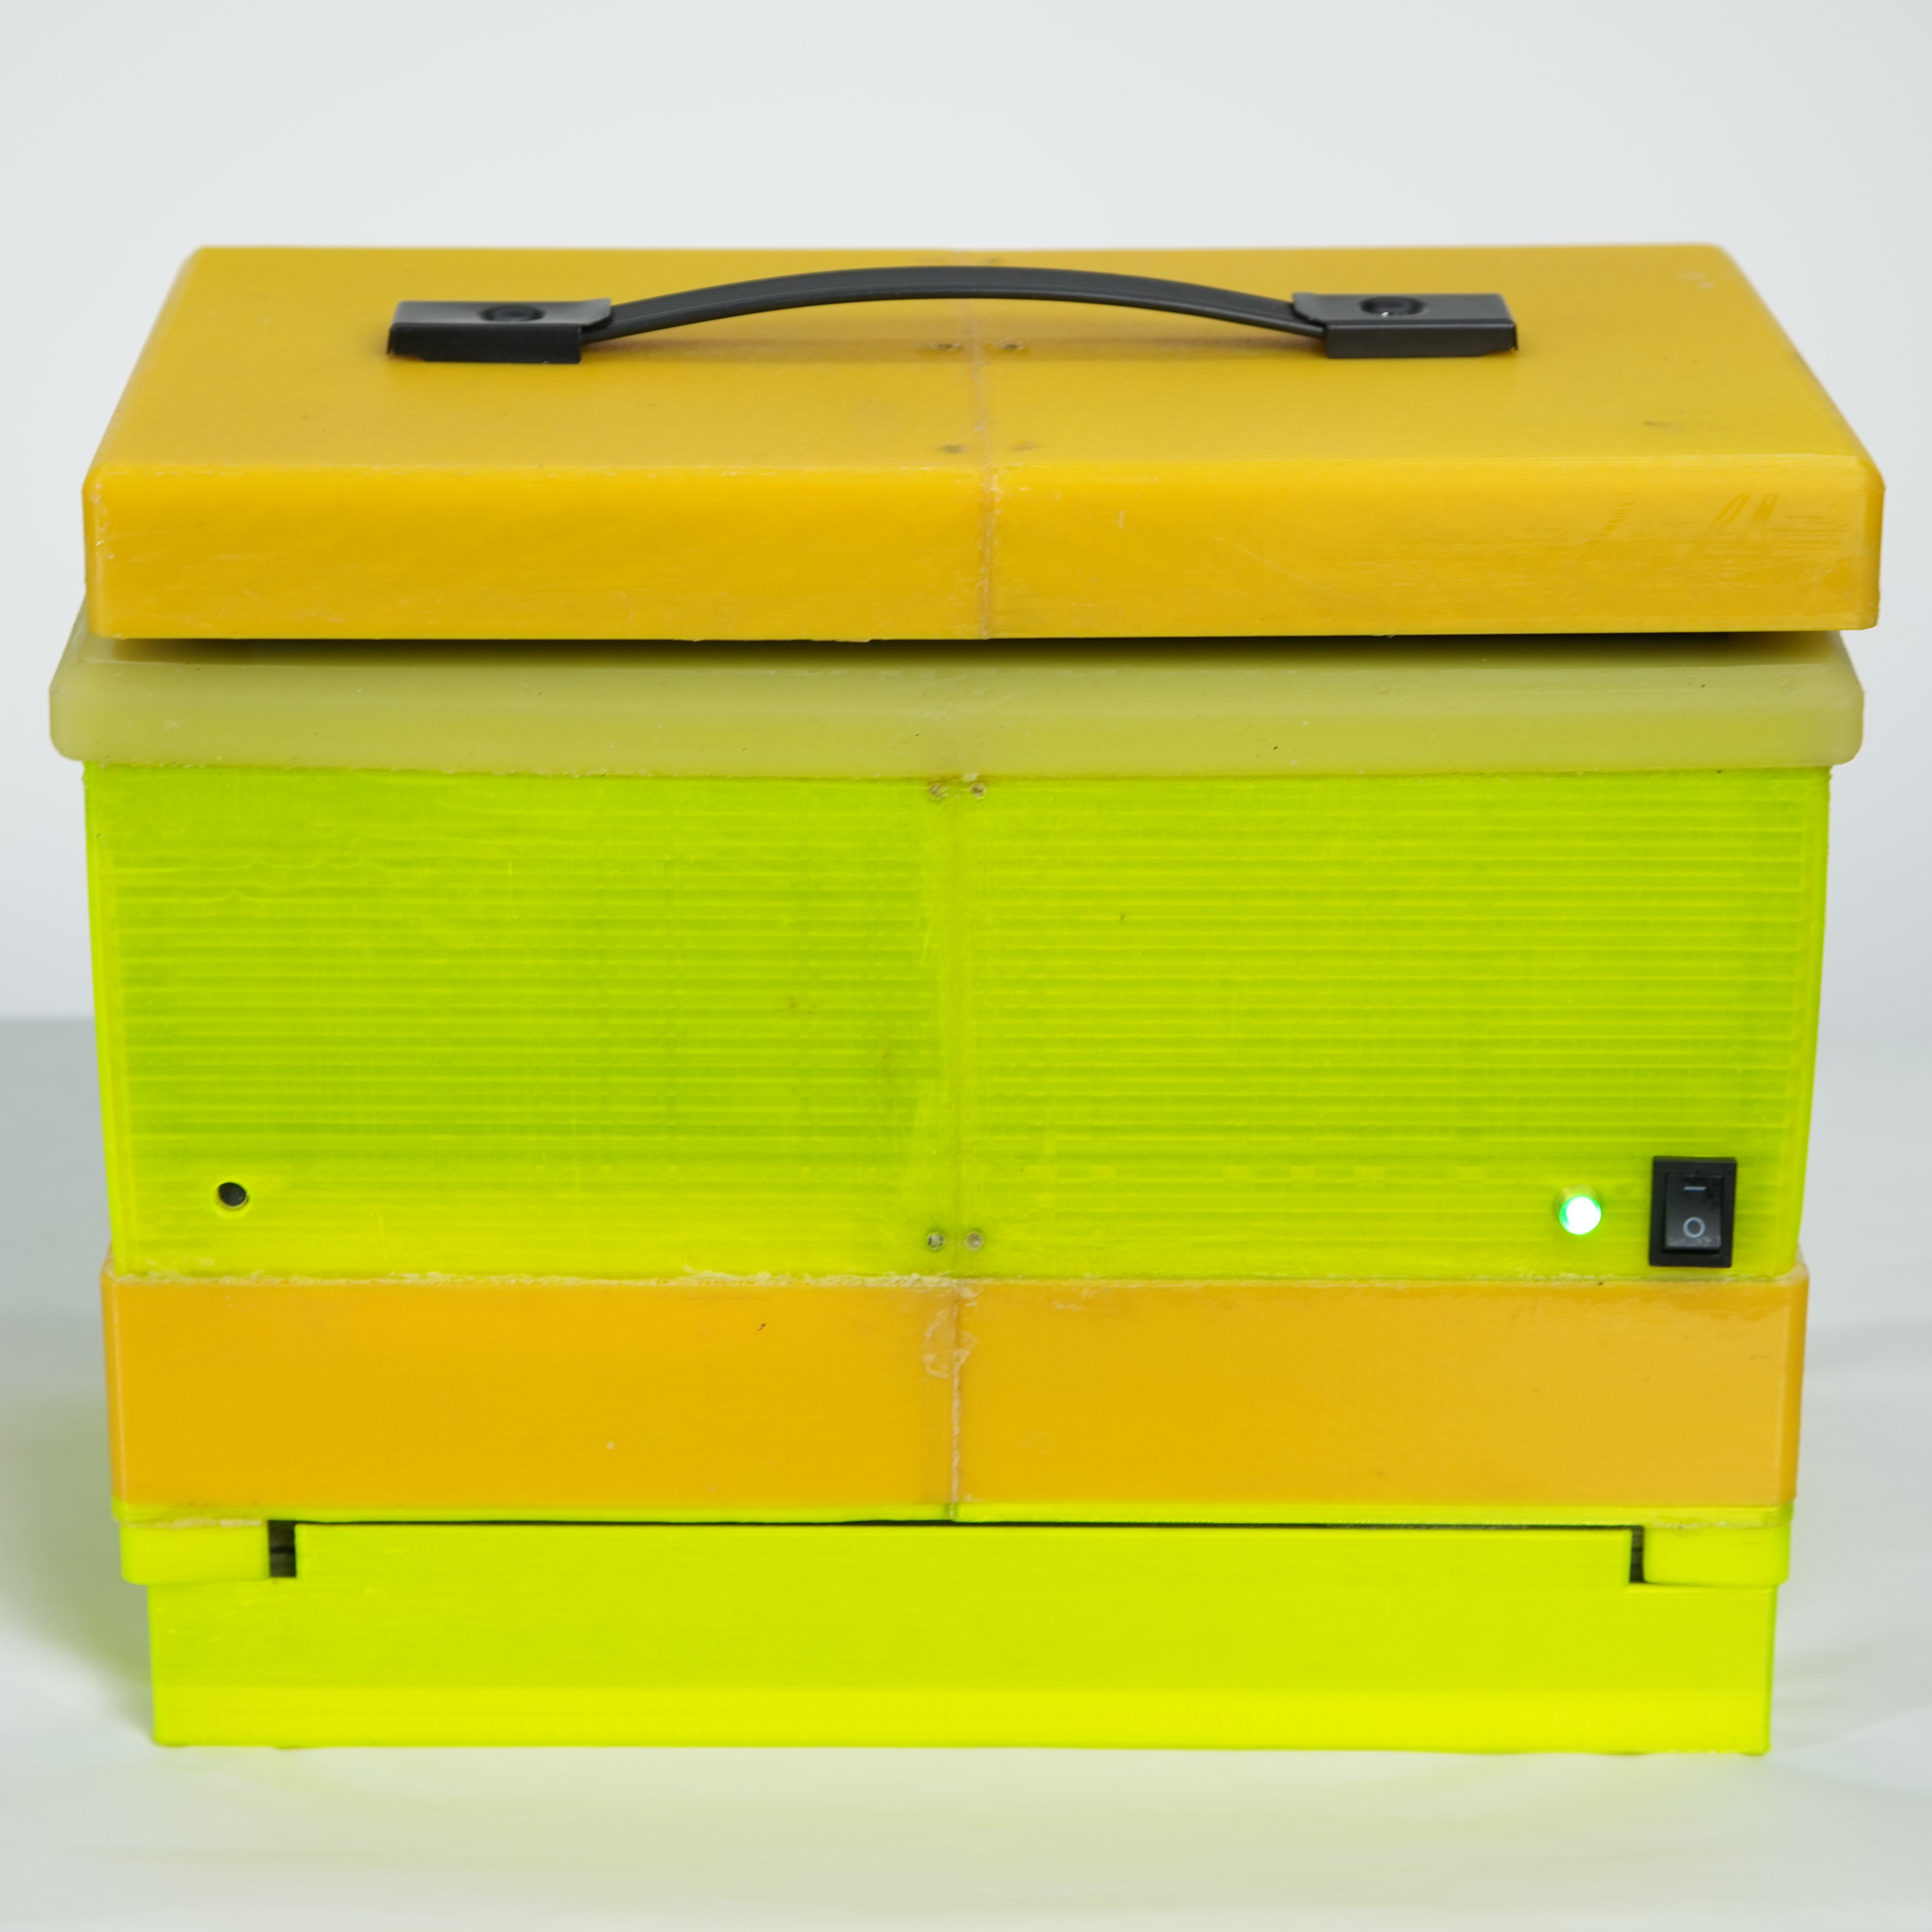
\includegraphics[width=\textwidth]{figures/methods/aspids1.jpg}
% 		\caption{Closed configuration}
% 		\label{fig:aspids_open}
% 	\end{subfigure}%
% 	\qquad
% 	\begin{subfigure}{0.45\textwidth}
% 		\centering
% 		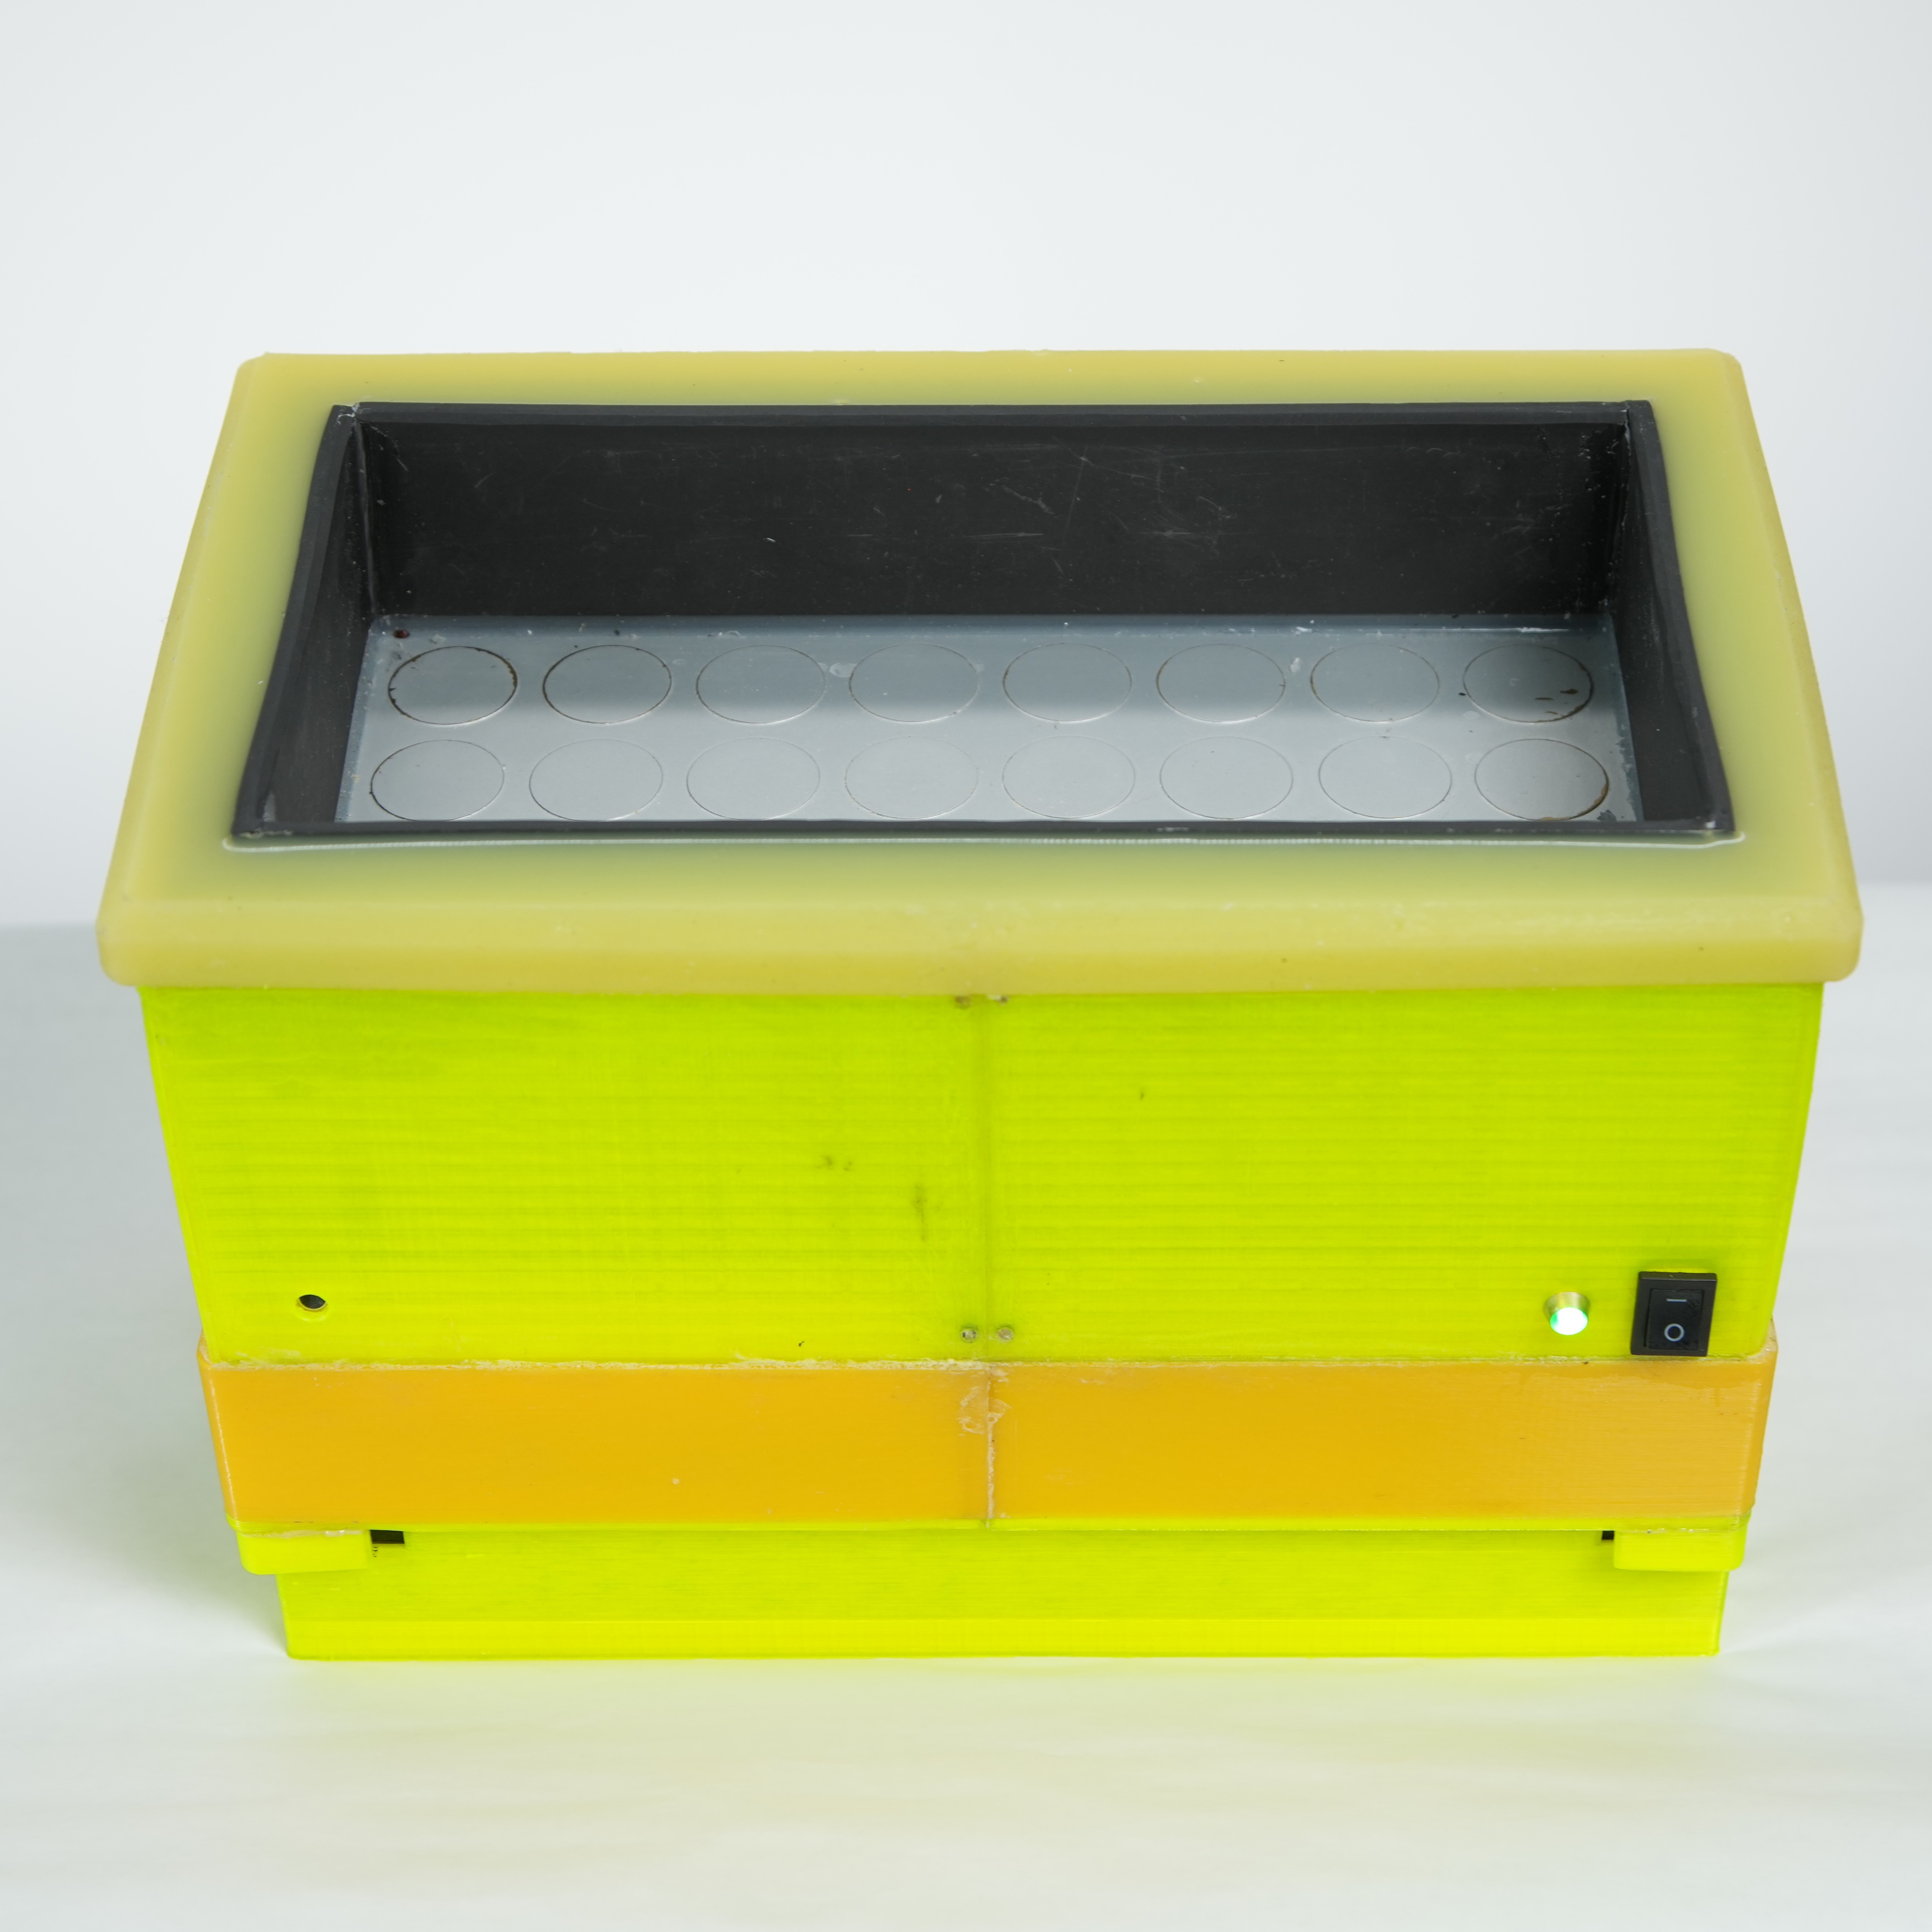
\includegraphics[width=\textwidth]{figures/methods/aspids2.jpg}
% 		\caption{Open configuration}
% 		\label{fig:aspids_closed}
% 	\end{subfigure}%
% 	\caption{A-SPIDS in (a) closed, (b) open configurations}%
% 	\label{fig:aspids_photos}
% \end{figure}

\newpage
\section{Tested Insect, Materials, and Noise Levels}

Although stored products insects proliferate across a wide range of commodities, they are difficult to obtain for research purposes. The cowpea beetle, \textit{Callosobruchus maculatus}, the confused flour beetle, \textit{Tribolium confusum}, and the mealworm and darkling beetle, \textit{Tenebrio molitor}, are commercially available and were chosen based on their similarities to the sizes, qualities, and behavior to the species targeted during inspection. Table \ref{tab:insects} provides a summary of the tested insect species.

% make the font smaller for the table
\begin{table}[!htbp]
% \small
	\caption{Description of tested live specimens \label{tab:insects}}
	\centering
    % \small
	\begin{tabular}{@{}llrrr@{}}
		\toprule
		\textbf{Scientific Name}  & \textbf{Common Name}  & \textbf{Size [\si{\milli\meter}]} & \textbf{Weight [\si{\milli\gram}]} & \textbf{Density [\si{\kilo\gram\per\liter}]} \\
		\midrule
		\textit{C. maculatus}     & Cowpea beetle         & \(4 \times 1 \times 1\)           & 2.1                                & 0.525                                        \\
		\textit{T. confusum}      & Confused flour beetle & \(4 \times 2 \times 2\)           & 1.0                                & 0.625                                        \\
		\textit{T. molitor}       & Darkling beetle       & \(15 \times 5 \times 3\)          & 160.0                              & 0.711                                        \\
		\textit{T. molitor} larva & Mealworm              & \(20 \times 2 \times 2\)          & 130.0                              & 1.625                                        \\
		\bottomrule
	\end{tabular}
\end{table}

The cowpea weevil or cowpea seed beetle and also known as the pulse beetle, \textit{Callosobruchus maculatus}, is part of the leaf beetle family, \textit{Chrysomelidae}, and infests cowpea and mung beans. Adults are small, round beetles, brownish with black, pale spots and stripes, and range from \SIrange{2}{4}{\milli\meter} in length. Adults have a lifespan of 12 days and colonies reproduce until their food supply is depleted. Females lay eggs on the surface of the beans. Upon hatching in around five days, larvae dig into the seed and feed on the cotyledons as they develop until they bore out of the bean as adults within 25-30 days \cite{tranConsequencesInbreedingCowpea1995}. This boring behavior is similar to other internal feeders, such as the lesser grain borer, \textit{R. dominica}, and the rice weevil, \textit{S. oryzae}, that are targeted as problematic by the USDA. Flying versions of the species can disperse to new locations, including directly to cowpea fields. Even a \SIrange{1}{2}{\percent} infestation on a field can result in \SI{80}{\percent} loss of product after six to eight months of storage. In West Africa, up to \SI{100}{\percent} loss was reported after several months of unmitigated infestation \cite{mohamedn.sallamInsectDamagePostHarvest2013}.

The confused flour beetle, \textit{Tribolium confusum}, is an arthropod that infests farinaceous products such as rice and flour. They are reddish-brown with clubbed antennas and range from \SIrange{2}{4}{\milli\meter} in length. As a secondary pest, the larvae and adult forms are found in damaged and processed grains. Their infestations often result in a grey tint, odor, production of toxic quinones, and encourage mold growth. The confused flour beetle eggs are white and microscopic, proving a challenge to detect among the material they settle. Their lifecycle takes 40 to 90 days and the adults are capable of living up to three years in moderate climate conditions \cite{mohamedn.sallamInsectDamagePostHarvest2013, baldwinConfusedFlourBeetle2020}.

The \textit{Tenebrio molitor} is known in its larval form as the mealworm and in its adult form as the darkling beetle. The larvae are \SIrange{1}{2}{\centi\meter} long, have a dark brown head, and a segmented yellow body with a hard exoskeleton. Adults also grow up to \SI{2}{\centi\meter} in length but are a shiny brown or black color. Females can lay up to 6000 eggs during their lifecycle. Darkling beetles release benzoquinones that result in an unpleasant odor \cite{mohamedn.sallamInsectDamagePostHarvest2013, vigneronImmuneDefensesBeneficial2019}.

% \begin{figure}[!htbp]
% 	\centering
% 	\begin{subfigure}{0.20\textwidth}
% 		\centering
% 		\includegraphics[width=\textwidth]{figures/methods/maculatus.jpeg}
% 		\caption{\textit{C. maculatus}}
% 		\label{fig:maculatus}
% 	\end{subfigure}%
% 	\qquad
% 	\begin{subfigure}{0.20\textwidth}
% 		\centering
% 		\includegraphics[width=\textwidth]{figures/methods/confusedflour.jpeg}
% 		\caption{\textit{T. confusum}}
% 		\label{fig:confusum}
% 	\end{subfigure}%
% 	\qquad
% 	\begin{subfigure}{0.20\textwidth}
% 		\centering
% 		\includegraphics[width=\textwidth]{figures/methods/darkling.jpeg}
% 		\caption{\textit{T. molitor}}
% 		\label{fig:darkling}
% 	\end{subfigure}%
% 	\qquad
% 	\begin{subfigure}{0.20\textwidth}
% 		\centering
% 		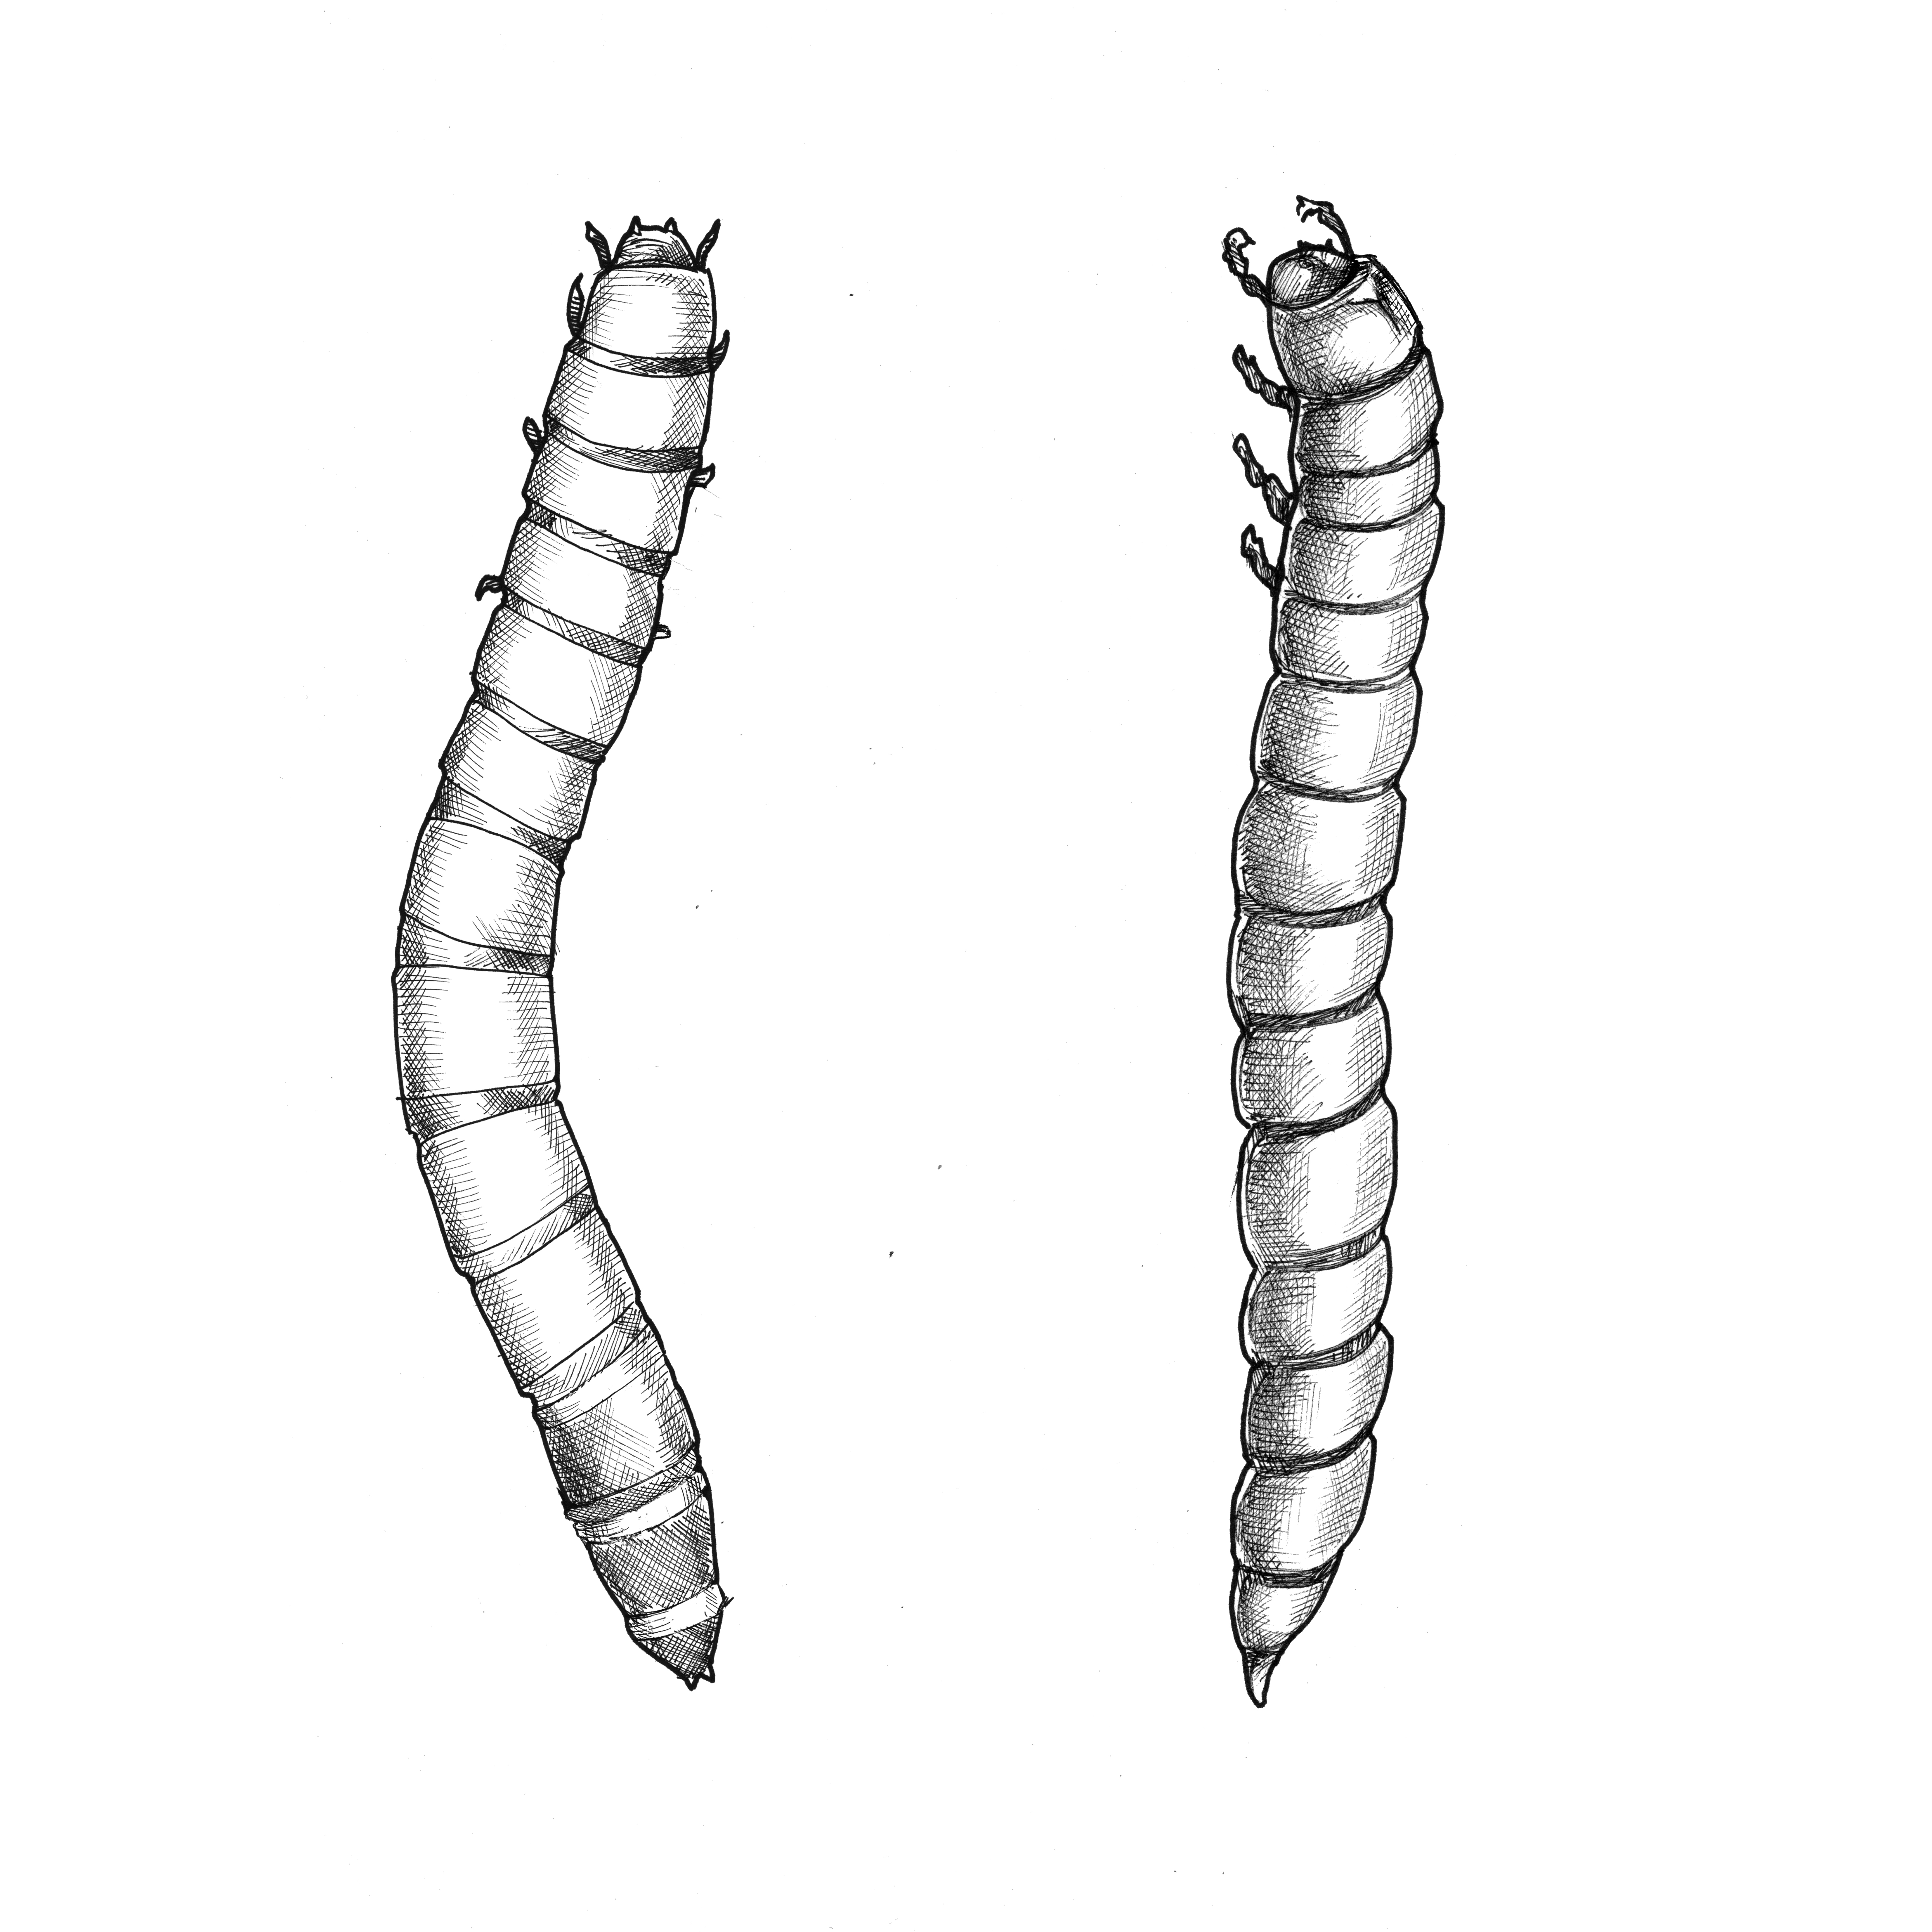
\includegraphics[width=\textwidth]{figures/methods/mealworm.jpg}
% 		\caption{\textit{T. molitor} larva}
% 		\label{fig:mealworm}
% 	\end{subfigure}%

% 	% \qquad
% 	\caption{Drawings of the insects.}%
% 	\label{fig:insect_drawings}
% \end{figure}

\newpage
A variety of stored product materials were tested with and without insect specimen including oatmeal, \textit{Avena sativa}, rice, \textit{Oryza sativa}, wheat in the form of whole groat kernels and processed flour, \textit{Triticum aestivum}, and corn in the form of Corn Flakes, \textit{Zea mays}. The material samples were kept in sealed storage containers to prevent contamination and infestation. During testing, \SI{1}{\liter} of clean material was transferred into a plastic bag and placed into the sensor container. After several minutes of silence were recorded to ensure the grains were settled, a single insect was introduced into the material. Table \ref{tab:recording} summarizes the duration of recordings for each insect-material pairing. The insect-material pairings are not fully balanced as a result of varying life stages and availability of the insects, the need to test in clean and uncontaminated materials, and the time and budget restraints of the project.

\begin{table}[!htbp]
	\caption{Duration of recordings in minutes for insect-material pairings with silence. The duration of recordings with external noise are accommodated with parenthesis. \label{tab:recording}}
	\centering
	\begin{tabular}{lrrrrr}
		\toprule
		                          & \textbf{\textit{A. sativa}} & \textbf{\textit{O. sativa}} & \multicolumn{2}{c}{\textbf{\textit{T. aestivum}}} & \textbf{\textit{Z. mays}}                \\
		                          & Oatmeal                        & White Rice                     & Wheat Groats                                            & Flour                      & Corn Flakes  \\
		\midrule
		\textit{C. maculatus}     & 12                             & 258 (12 noise)                 & 13                                                      & 20 (1 noise)               & 17           \\
		\textit{T. confusum}      & 39                             & 274 (16 noise)                 & 189                                                     & 55 (1 noise)               & 16           \\
		\textit{T. molitor}       & 68                             & 15                             & 9                                                       & 8                          & 13           \\
		\textit{T. molitor} larva & 46 (4 noise)                   & 268 (132 noise)                & 51 (2 noise)                                            & 128                        & 43 (5 noise) \\
		\midrule
		No insect                 & 4                              & 219 (64 noise)                 & 142 (2 noise)                                           & 24                         & 23           \\
		\bottomrule                                                                                                                                                                                       \\
	\end{tabular}
\end{table}

The expected usage of the system would be within a variety of environments such as storage facilities, warehouses, and ports, where machinery, vehicles, and people can create significant background noise. The sound pressure levels can range from \SIrange{35}{50}{\deci\bel A}, common for an office, up to \SI{110}{\deci\bel A} such as a factory \cite{mankinPerspectivePromiseCentury2011,claudiaNoiseSourcesCharacterization2012}. The system was exposed to varying levels of natural and simulated, ambient and artificial noise with and without live insect specimens to examine the efficacy of the sound insulation as well as the influence on the detection, false positive, and false negative performance. The ambient noise was a result of the surrounding laboratory environment including equipment, HVAC units, and personnel as well as vehicular and aircraft traffic. Artificial noise, such as pre-recorded sweeps, white noise, loud conversations, crowds, and factory noise were played through a speaker system at increased steps from \SIrange{60}{110}{\deci\bel A} and the noise levels were measured using a calibrated sound level meter, the Extech 407730 Digital Sound Level Meter manufactured by Teledyne FLIR \cite{sonically_soundCrowdCafeteria2022,viertelnachvierFactory22014,inspectorjAmbienceMachineFactory2017, EXTECH407730Digital}.

\newpage
\section{Stored Product Insect Database (SPIDB)}

The Stored Product Insect Dataset (SPID) is a repository of audio recordings collected by the Stored Product Insect Detection System. The dataset features the audio recordings as well as metadata describing the recording system, noise conditions, insect species, and material substrates. The full \SI{100}{\giga\byte} dataset can be downloaded from Kaggle \cite{danielkadyrovStoredProductInsecta}. An excerpt of the dataset file structure is shown in Listing \ref{lst:spid_directory}:

\begin{listing}[htbp]
	\caption{File organization of the Stored Product Insect Dataset \label{lst:spid_directory}}
	\begin{minted}{text}
\---data
¦   spi.db
¦  
+---aspids
¦   ¦   aspids_log.csv
¦   ¦   
¦   +---2023
¦   ¦   ¦   +---24
¦   ¦   ¦   ¦   +---2023_05_24_19_41_19.559_t00100
¦   ¦   ¦   ¦   ¦       2023_05_24_19_41_19.559_t00100_Ch0_00001.wav
¦   ¦   ¦   ¦   ¦       2023_05_24_19_41_19.559_t00100_Ch0_00002.wav
	\end{minted}
\end{listing}

The audio recordings are organized by date and the file names describe the recording date, time, a string descriptor, sensor channel, and recording iteration. The filename is structured as follows: \texttt{YYYY} is the four-digit year, \texttt{MM} is the two-digit month, \texttt{DD} is the two-digit day, \texttt{HH} is the two-digit hour in 24-hour format, \texttt{MM} is the two-digit minute, \texttt{SS.fff} is the seconds and milliseconds, \texttt{ssssss} is a string descriptor of the recording conditions, \texttt{Ch\#} is the sensor channel number, and \texttt{iiiii} is the five-digit recording iteration. The file name structure is detailed in Listing \ref{lst:filename}. 

\begin{listing}[htbp]
	\caption{File organization of the Stored Product Insect Dataset \label{lst:filename}}
	\begin{minted}{text}
YYYY_MM_DD_HH_MM_SS.fff_ssssss_Ch#_iiiii.wav
	\end{minted}
\end{listing}

The Stored Product Insect Database (SPIDB) provides an interface to access the data collected from the A-SPIDS platform. Acoustic data requires a rich set of metadata to provide context. This could range from information about the recording system such as the sensor type and sensitivity, environmental conditions such as background noise levels and descriptions, as well as details about the featured subjects. Commonly, datasets, like BugBytes, provide acoustic data as a set of audio files along with text-based files annotating each recording. Even when data is provided, it is often decoupled and requires significant effort to match the audio.

\newpage
SPIDB is a fork of the Sound Organization for Network Integration and Collection/Collaboration (SONICDB) framework, which was developed to address the challenge of organizing and sharing acoustic data when large amounts of associated metadata are required for analysis and interpretation \cite{rochManagementAcousticMetadata2016}. SONICDB leverages relational databases to link audio files with their corresponding minutiae, enabling efficient data management and retrieval as well as simplified sharing across different users and computers. Although any database reader or programming language can be used to interact with a database, an object-oriented wrapper was developed in Python using industry standard packages and methods. This interface was used to directly write A-SPIDS data to the database as well as throughout the data processing and analysis pipeline. Currently, the database is a locally stored SQLite file, which can be easily version-controlled and distributed. The interface can also support server-based SQL database systems such as MySQL and PostgreSQL.

Installing the SPIDB package can be performed through the Pip Installs Packages (PIP) Python package manager or by directly downloading from the GitHub repository. The dataset can be downloaded directly from Kaggle or using a script that is provided with the SPIDB package. Listing \ref{lst:spidb_install} describes the commands to install the SPIDB package and utilize package to download the dataset.  

\begin{listing}[htbp]
	\caption{Installing SPIDB package and downloading the database \label{lst:spidb_install}}
	\begin{minted}{bash}
# Install the SPIDB package
pip install spidb 
# Create a directory 
mkdir spid 
# Download the SPIDB database into the spid directory
spidb download --output-dir spid 
	\end{minted}
\end{listing}

SONICDB initializes with several preliminary models. The \texttt{File} model represents the audio files stored in the database, detailing the filepath, filename, extension, sample rate, duration, start and end time, as well as the sensor and channel the files were recorded with. The sensor and channel properties are directly tied to the \texttt{Sensor} and \texttt{Channel} models, respectively. The \texttt{Sensor} model categorizes the name, subname, manufacturer, sensor type, and number of channels of the sensor as well as a list of associated \texttt{Channel} and \texttt{File} entities. The \texttt{Event} model facilitates storing details of the logged events, including start and end times, description, noise levels, and the associated \texttt{Material} and \texttt{Subject} entities. The \texttt{Subject} model captures information about the subjects being recorded. SPIDB extended it to include bespoke attributes such as scientific name, common name, weight, height, length, width, volume, and density. SPIDB also added the \texttt{Material} model to describe the substrate in which the subjects are placed. 

\newpage
Figure \ref{fig:spidb} shows the schema for the SPIDB:

\begin{figure}[!htbp]%
	\centering
	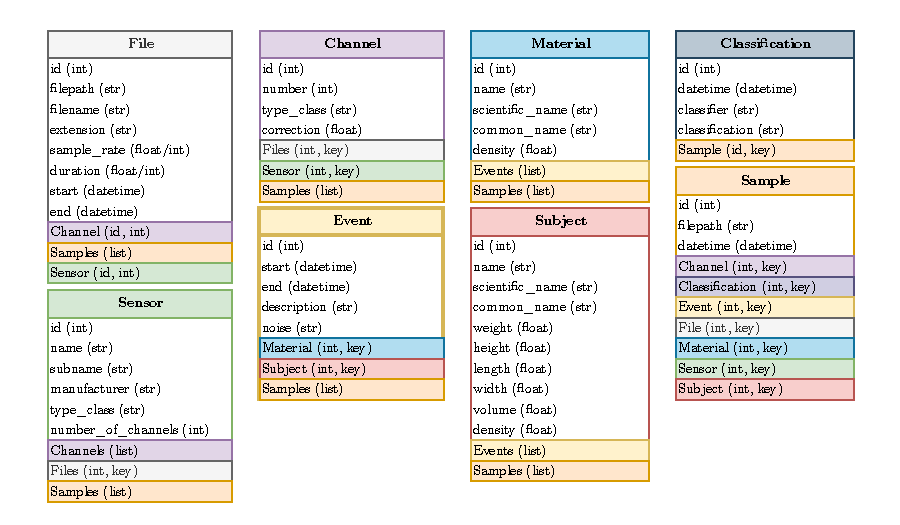
\includegraphics[width=\textwidth]{figures/methods/database_diagram.pdf}
	\caption{Schema of the Stored Product Insect Database (SPIDB)}%
	\label{fig:spidb}%
\end{figure}

SONICDB uses popular and standard Python packages ensuring standardized database management and coding conventions. SQLAlchemy allows defining the database schema using Python classes, making it easier to interact with the database using an object-oriented approach. Additionally, Alembic is used for database migrations, enabling version control for the database schema \cite{fredstamComparingDatabaseManagement}. The data is extracted as Pandas DataFrames and Numpy Arrays. Audio data is handled through Librosa and PyDub. Listing \ref{lst:spidb_connection} shows an example of connecting to the database using Python once the dataset is downloaded and the user is within the directory containing the database file, \texttt{spi.db}:

\begin{listing}[htbp]
	\caption{Example of connecting to the SPIDB using Python \label{lst:spidb_connection}}
	\begin{minted}{python}
from spidb import spidb 

db = spidb.Database("spi.db")
	\end{minted}
\end{listing}

\newpage
Once available, a user can interact with the database using the defined models and perform various operations such as querying, inserting, updating, and deleting records. Listing \ref{lst:spidb_query} shows an example of querying the database for all the tested materials and then retrieving all recordings where the material is associated with a specific insect species, \textit{C. maculatus}:

\begin{listing}[htbp]
	\caption{Example of querying the SPIDB for a specific insect species \label{lst:spidb_query}}
	\begin{minted}{python}
# Query for all tested materials
materials = db.Material.query.all() #[Material <id>, ...]

# Retrieve all events for a specific insect species
species = "Callosobruchus maculatus"
events = db.session.query(spidb.Event).filter(
    spidb.Event.subject.name == species
    ).filter(
        spidb.Event.material.id.in_([m.id for m in materials])
    ).all() # [Event <id>, ...]
	\end{minted}
\end{listing}

Although the audio can be retrieved by accessing the \texttt{File} entity, independently or through association to the \texttt{Event}, \texttt{Sensor}, or \texttt{Channel} entities, SONICDB provides an accessible method to retrieve the data if the start, end, and channel are known. Listing \ref{lst:sonicdb_retrieval} shows an example of how to retrieve audio data from SONICDB.

\begin{listing}[htbp]
	\caption{Example of retrieving audio data from SONICDB \label{lst:sonicdb_retrieval}}
	\begin{minted}{python}
# Retrieve the Event entity for which audio is to be extracted
event = db.session.query(spidb.Event).one() # <Event id>

# Retrieve audio from channel 2 for the duration of the event
audio = db.get_audio(
    event.start,
    event.end,
    sensor=event.sensor,
    channel_number=2
) # <Audio id>
	\end{minted}
\end{listing}

The code used to generate the data and figures in this report is available in the appendix and the accompanying GitHub repository. The full documentation, including examples and scripts, for SONICDB and SPIDB is available on GitHub \cite{danielkadyrovDkadyrovSpidbSPIDB2024}.

\newpage